\begin{document}
\sectiontitle{7}{Open-Loop Stimulation Sequence}
\setstretch{1.6}
The open loop stimulation sequence specifies which muscles should be stimulated, the duration of their activation and the delays between activations. The sequence aims to replicate a single step (gait cycle) for one leg using FES. The final goal is to produce a step that feels and looks natural and is comfortable for the subject while being general enough to work for a variety of subjects.

\subsection{Methods}
\subsubsection{Electrode Placement}
The placement of electrodes is an critical factor for achieving effective stimulation. It determines the quality of muscle activation the specificity and the comfort for the user\todo{source}. However, the optimal placements for each muscle is highly subject-dependent \todo{source} which makes the process of finding the placements both challenging and time consuming.

To establish some form of systematic approach the optimal placements were first found in myself. This involved iteratively adjusting the placement of both the active and reference electrode positions, observing the muscle responses at different amplitudes and the discomfort level until a functional movement was achieved under the pain threshold (maximum tolerable intensity). Physiologically, optimal electrode placement aligns with the motor points of the targeted muscles \cite{gobbo_muscle_2014}. Motor points are regions where the motor nerve enters the muscle, resulting in the lowest threshold for activation thus minimizing discomfort and fatigue \cite{gobbo_muscle_2014}. To find the optimal placements for each muscle several sources were consulted with the most used source being an atlas of the muscle motor points by A. Botter \cite{botter_atlas_2011}. 

\begin{figure}
    \centering
    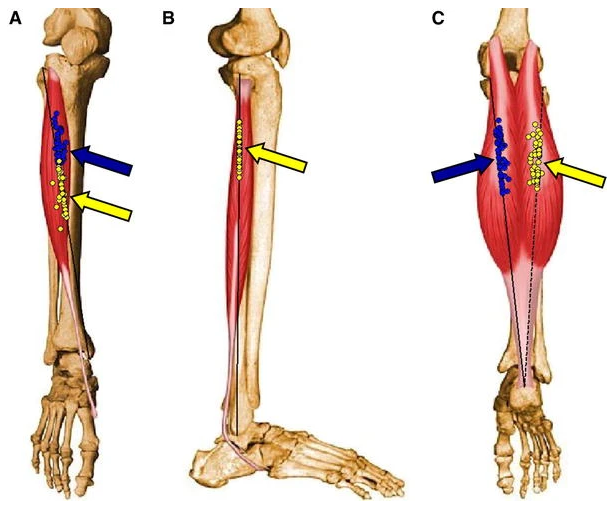
\includegraphics[width=0.6\linewidth]{images/screenshotmotorpoint.png}
    \caption{Example of motor points according to \cite{botter_atlas_2011} for: \textbf{a.} tibialis anterior; \textbf{b.} peroneous longus; \textbf{c.} medial (\textit{blue circles}) and lateral (\textit{yellow circles}) gastrocnemii. }
    \label{fig:motor-points}
\end{figure}

To document the process and provide a reference for future users a series of videos was created, where each video captures the intended functional movement elicited by optimal stimulation of a muscle. This offers a clear visual benchmark which could then be used when finding the correct placements for new users, thereby maintaining consistency and ensuring that the functional movements are sufficient before moving on to the full gait cycle functional electrical stimulation.

\subsubsection{Analysis of the Initial Sequence}
Initially, it was believed that a working open loop sequence had already been established by a previous student. The original intended methodology for the open loop sequence was therefore to merely validate it's functioning in two subjects. 

Once it became clear that the sequence was not functioning as expected, it was decided to identify the cause of the problem before attempting to create a new sequence. Several potential reasons for the failure were considered: incorrect stimulation intensity, improper electrode placement, issues with the software implementation, or flaws in the sequence itself.

To address potential problems related to electrode placement and stimulation intensity, an experienced colleague supervised the process to ensure optimal placement and settings. Adequate time was devoted to finding the best configurations for both.

Next, the software implementation was validated by testing the sequence without a subject. This involved verifying that the correct channels were activated at the appropriate intensities, durations, and times.

After ruling out these factors, the only remaining potential issue was the sequence itself. The methodology used to develop the sequence was analyzed, along with the accuracy and reliability of the EMG data it was based on. This data was then compared with more reliable open-source data to further investigate the sequence's validity.


\subsubsection{Designing a New Sequence}
In order to design a new sequence that would be robust insights from the literature relating to FES for gait and a seminal text on gait physiology were used. To ensure that the sequence aligned with natural muscle activation patterns, the seminal text \textit{Gait Analysis: Normal and Pathological function} \cite{perry_gait_2024} was consulted. This book provides comprehensive descriptions of muscle activity throughout the gait cycle with exact start and stop activation percentages of the gait cycle for nearly all lower extremity muscles during gait. However, the stimulation sequence could not only be based on this. FES does not have the necessary selectivity in order to stimulate every lower extremity muscle individually as they are activated naturally during gait. Unlike voluntary contractions, which selectively and smoothly activate specific motor units, FES broadly stimulates motor nerves, often activating muscles indiscriminately \todo{source}. It was therefore necessary to choose only a few muscles to stimulate. Existing literature relating to FES was consulted for this purpose.



\subsubsection{Validation of the Final Sequence}
The final four muscle open loop stimulation sequence was tested on three healthy subjects between the ages of 22 and 25, two female and one male. This was done before moving further with closed loop development, to ensure that the stimulation sequence was generalizable across individuals. During the setup phase the optimal placements for the electrodes for each individual subject were found along with the motor threshold and the maximum tolerable intensity. The stimulation intensity was set as the value in which the functional movement associated with that muscle was achieved and the movement resembled the reference videos mentioned in the methods section as closely as possible.

The subjects were then fitted with the Xsens Awinda  motion capture system IMUs. The Xsens Awinda is a wireless, wearable system that uses IMUs specifically designed to capture human movement without the need for cameras or external markers \cite{noauthor_mvn_nodate}. It is often used for validation in literate since it provides accurate, portable motion tracking. The system was calibrated before subjects were instructed to go on the treadmill. 

\todo{XSens figure}

The treadmill was set to 1.5km/h and subjects were instructed to relax as much as possible the muscles in the leg which would be stimulated. The stimulation ran for 3 minutes and thereafter a baseline measurement was done in which the subjects muscles were not stimulated and they simply walked on the treadmill for three minutes. 


\subsection{Implementation}
\subsubsection{Analysis of the Initial Sequence}
\begin{wrapfigure}{r}{0.3\textwidth} 
    \centering
    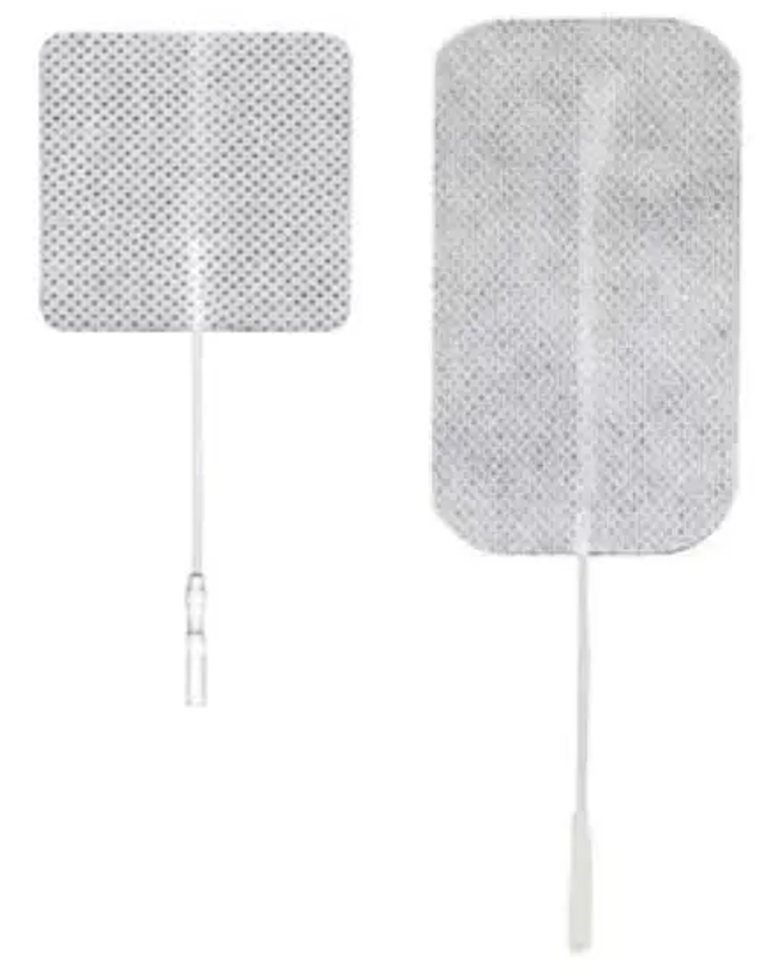
\includegraphics[width=\linewidth]{images/electrodes.png}
    \caption{FES electrodes}
    \label{fig:electrodes}
\end{wrapfigure}
In order to realize the connection between the StimWave and the muscles every stimulated muscle required two electrodes, one active electrode and one reference electrode. Both 5x5cm and 5x9cm electrodes were used for this project (figure \ref{fig:electrodes}), depending on the muscle size. The connection was realized using cables with banana connectors, visible in figure \ref{fig:stimwave}. The chosen electrodes are equipped with adhesive gel, creating a relatively stable electrode-tissue interface. These are the electrodes used for the testing of the initial sequence, but also for all subsequent stimulation setups.

\subsubsection{Designing a New Sequence}
\begin{figure} [h]
    \centering
    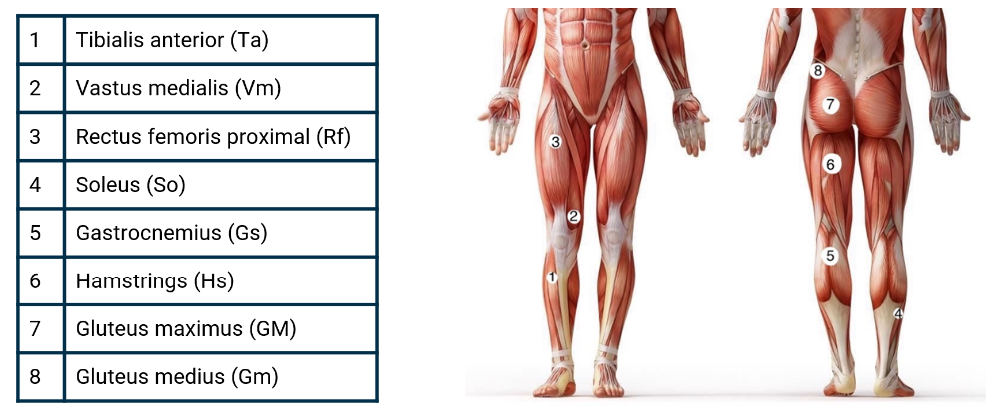
\includegraphics[width=0.85\linewidth]{images/common_muscles.png}
    \caption{Common muscles used for FES driven gait}
    \label{fig:commonMuscles}
\end{figure}

The literature, e.g. \cite{aout_effects_2023}, \cite{chaikho_transcutaneous_2022} and the sources therein, revealed a large variety in the sequences used in FES gait studies. The timing end exact muscles varied greatly, however, the number of muscles was relatively consistent between four and eight and the tibialis anterior, gastrocnemis and biceps femoris (hamstring) appeared consistently in nearly all implementations. A list and visualization of the most common muscles is shown in figure \ref{fig:commonMuscles}. Several sequences inspired by physiological insights and the literature were tested. Specifically three configurations with six, five and four muscles are discussed in the corresponding results section. 

To facilitate the testing and tuning of new stimulation sequences a new graphical user interface (GUI) tab (figure \ref{fig:sequenceGUI})was created. This interface allowed real-time adjustments not only to the durations and delays but also the sequence of muscles. This is done by relating each muscle to a specific channel. This significantly accelerated the iterative process of testing and tuning sequences. 

\begin{figure} [h]
    \centering
    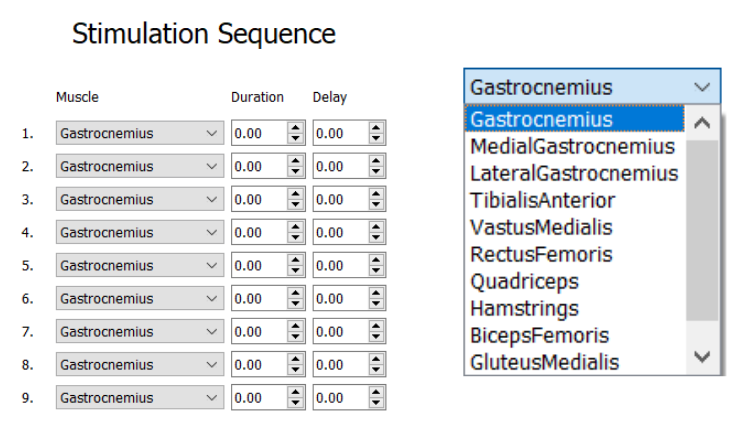
\includegraphics[width=0.8\linewidth]{images/sequenceGUI.png}
    \caption{Graphical user interface for modifying and testing new sequences.}
    \label{fig:sequenceGUI}
\end{figure}

\subsubsection{Validation of the Final Sequence}
To analyze the results of the stimulation experiment, data from the MVNX files produced by the Xsens system were processed in Python to extract and compare the knee angles across gait cycles with and without stimulation. The Xsens system includes inbuilt sensor fusion capable of outputting the knee angle this was then loaded for processing by using the \texttt{load\_mvnx} library. 

To align and normalize the gait cycles, the peaks in the knee flexion data were identified using the \texttt{scipy.signal} module. Consecutive peaks were used to segment the flexion data into individual gait cycles. To ensure meaningful averaging across cycles, the segmented gait cycles were normalized in length. Each cycle was interpolated to 100 equidistant points, corresponding to a percentage of the gait cycle. Once normalized the gait cycles were averaged point by point to compute the mean knee angle and standard deviation. The data was then shifted so that the peak would be centered at the 75\% mark. The standard deviation values were used to create the upper an lower bounds of the colored regions around the mean which is plotted as a continuous curve. 

\subsection{Results}

\subsubsection{Analysis of the Initial sequence}
Upon testing the initial sequence on two  subjects it became clear that the sequence was ineffective and did not produce a step. The muscle activation was observed to feel unnatural, uncomfortable and ultimately failed to replicate a smooth coordinated movement. It therefore became necessary to determine whether these issues stemmed from errors in the implementation or from issues with the sequence itself.

\begin{figure} [h]
    \centering
    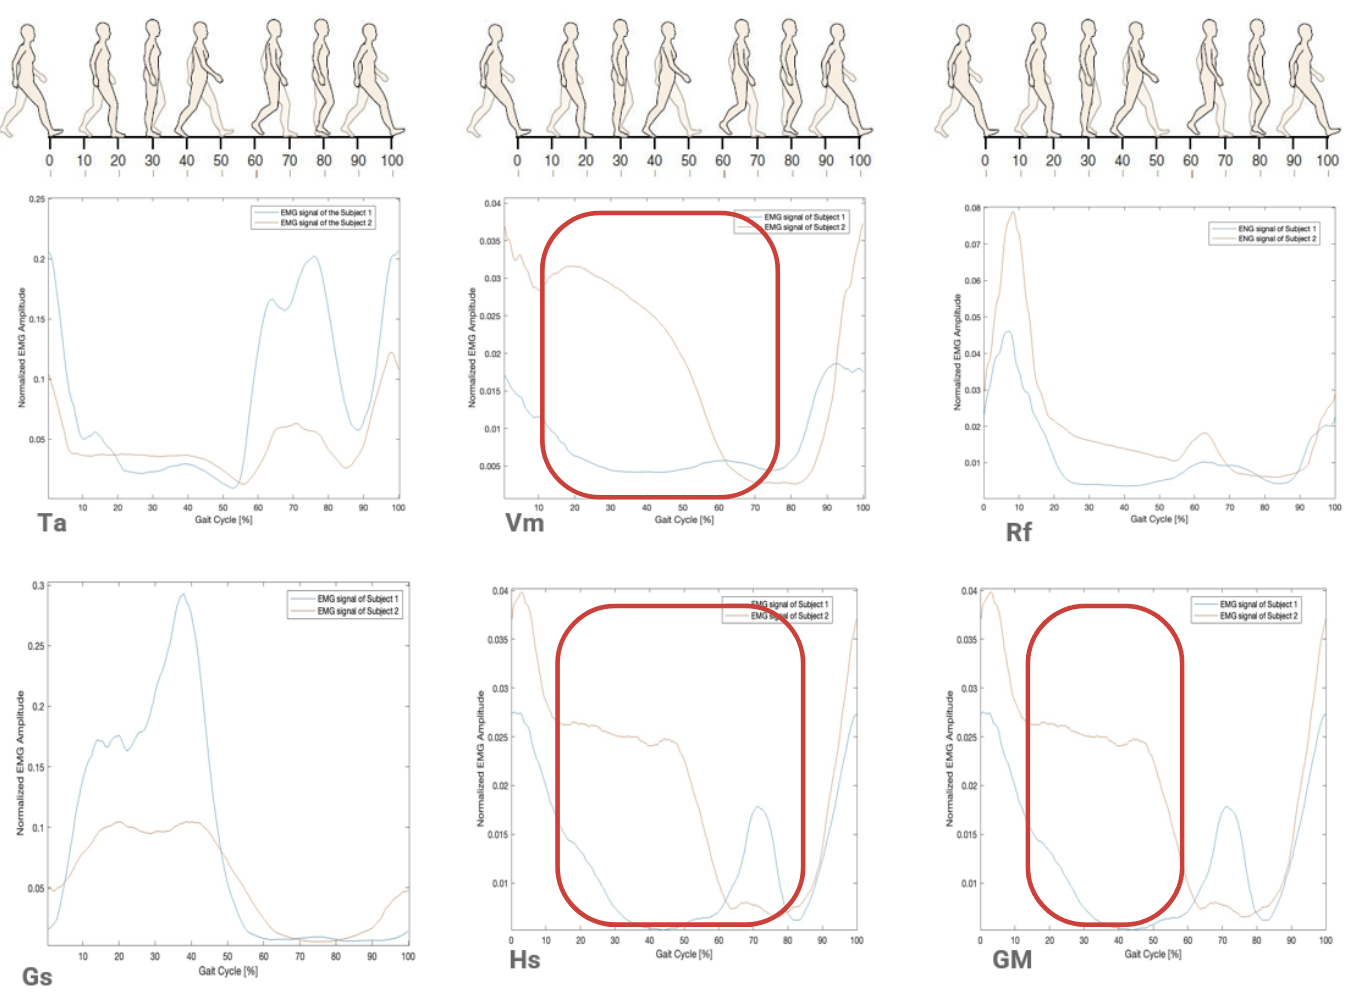
\includegraphics[width=0.99\linewidth]{images/wrongemg.png}

    \caption{EMG measurements from two subjects used by a previous student to determine the initial stimulation sequence. Highlighted inside the red boxes are the portions of the gait cycle in which there is an erroneous measurement of muscle activation. This ultimately lead to the development of an inaccurate stimulation sequence. (\textbf{Ta} - Tibialis Anterior, \textbf{Vm} - Vastus Medialis, \textbf{Rf} - Rectus Femoris, \textbf{Gs} - Gastrocnemius, \textbf{Hs} - Hamstrings, \textbf{GM} - Gluteus Maximus)}
    \label{fig:wrongemg}
\end{figure}

This initial sequence was based on electromyography (EMG) measurements of muscle activation during gait in two healthy subject. Therefore to evaluate the accuracy of the sequence the EMG measurements from the two subjects were compared against a comprehensive, open-source dataset of EMG activity during gait \cite{camargo_comprehensive_2021}. The discrepancies between the two became immediately apparent. In gait phases where the open-source dataset indicated that certain muscles-such as the vastus medialis, hamstrings, and gluteus maximus should be largely inactive the EMG measurement from the two subjects showed significant activation, as can be seen in figure \ref{fig:wrongemg}.Having confirmed that the issue lay in the sequence itself, rather than its implementation, the focus was then shifted to designing an entirely new stimulation sequence.

\subsubsection{Designing a New Sequence}

\paragraph*{Six Muscle Sequence}
First a sequence with six muscles: Tibialis Anterior, Gastrocnemi, Vastus Medialis, Hamstrings, Rectus Femoris and the Gluteus Maximus, was tested. This was the first sequence that produced a step. However, it had some limitations. Firstly, the use of six muscles creates a challenging setup, since determining electrode placements and stimulation intensity is a time consuming process. Secondly, even though the stimulation parameters were fine during the setup when one muscle is stimulated at a time, the sequence was noted to be uncomfortable, possibly because of the multitude of stimulation sites. Finally, the sequence appeared to produce some slight instability in the hip joint, possibly due to the joint stimulation of the rectus femoris, hamstrings and gluteus maximus, which all have an affect on hip extension \todo{source}.

\paragraph*{Five Muscle Sequence}
The next sequence did not include the gluteus maximus, this was done in order to determine whether it was a necessary muscle to stimulate. It had been pointed out by colleagues experienced with running FES on subjects that patients typically find the stimulation and placement process for the gluteus to be both challenging and uncomfortable. 

The hypothesis was that the gluteus maximus may not be necessary to stimulate since several studies using FES to produce gait did not include the gluteus muscles \cite{aout_effects_2023}. There are several reasons as to why the gluteus maximus, although important in natural gait, may not be necessary to stimulate. The first is muscle compensation. The gluteus is mostly involved in hip stabilization and hip extension. However the hamstring stimulation provides some hip extension that may be sufficient \cite{kang_activation_2013}. The second is that the gluteus is primarily active during activities that require powerful hip extension such as climbing stairs or running \cite{noauthor_gluteus_nodate}. For flat ground however, especially at slower speeds the gluteus may play a smaller role.

This new sequence also produced a step that was not of a lower quality than the sequence that included the gluteus. Stimulation was also noted to be more comfortable and seemed more stable without the gluteus, therefore it was decided that the gluteus could be removed from the sequence.

\paragraph*{Four Muscle Sequence}
Next a sequence without the Rectus Femoris was tested, this was done due to several observations. Firstly, during experiments it was observed that stimulating only the vastus medialis led to a full knee extension leading to questions as to why the rectus femoris must be stimulated as well. The rectus femoris functions in both hip flexion and knee extension during natural gait \todo{source}, however upon FES stimulation it was observed to mostly produce an extension. So a hypothesis was formed that the necessary knee extension may be achieved through stimulation of only the Vastus Medialis, which focuses solely on knee extension without impacting hip movement. 

Secondly, during testing in one healthy subject it proved difficult to find a comfortable electrode placement for rectus femoris. It also proved to be the most uncomfortable muscle to stimulate. This was corroborated as a typical experience among patients by experienced colleagues. 

Finally it was observed that there is a large discrepancy in when the rectus femoris is stimulated in the literature, compared to when it is active during natural gait. In fact, in the literature it was largely being used for knee extension, while physiologically this muscle is mostly active during the initial-swing and mid-swing phases where it provides foot clearance and does not act as an extensor at all. 

\begin{figure} [h]
    \centering
    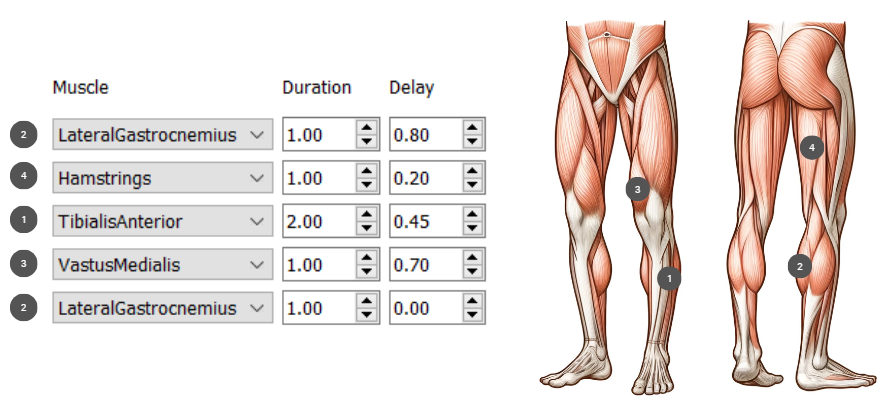
\includegraphics[width=0.99\linewidth]{images/final_seq_w_muscles.png}
    \caption{Final open-loop sequence along with an illustration of the final muscles chosen}
    \label{fig:fianlsequence}
\end{figure}

When comparing videos of the new sequence compared to the five muscle sequence, no discernible differences were found. The sequence also proved to be more comfortable, leading to the conclusion that rectus femoris may be removed from the sequence. This led to the choice of the final sequence visualized in figure \ref{fig:fianlsequence}. In order to ensure that the sequence was generalizable across individuals it was then tested in three subjects, with results available in the result section on the open-loop sequence.

\subsubsection{Validation of the Final Sequence}
\begin{figure}[h]
    \centering
    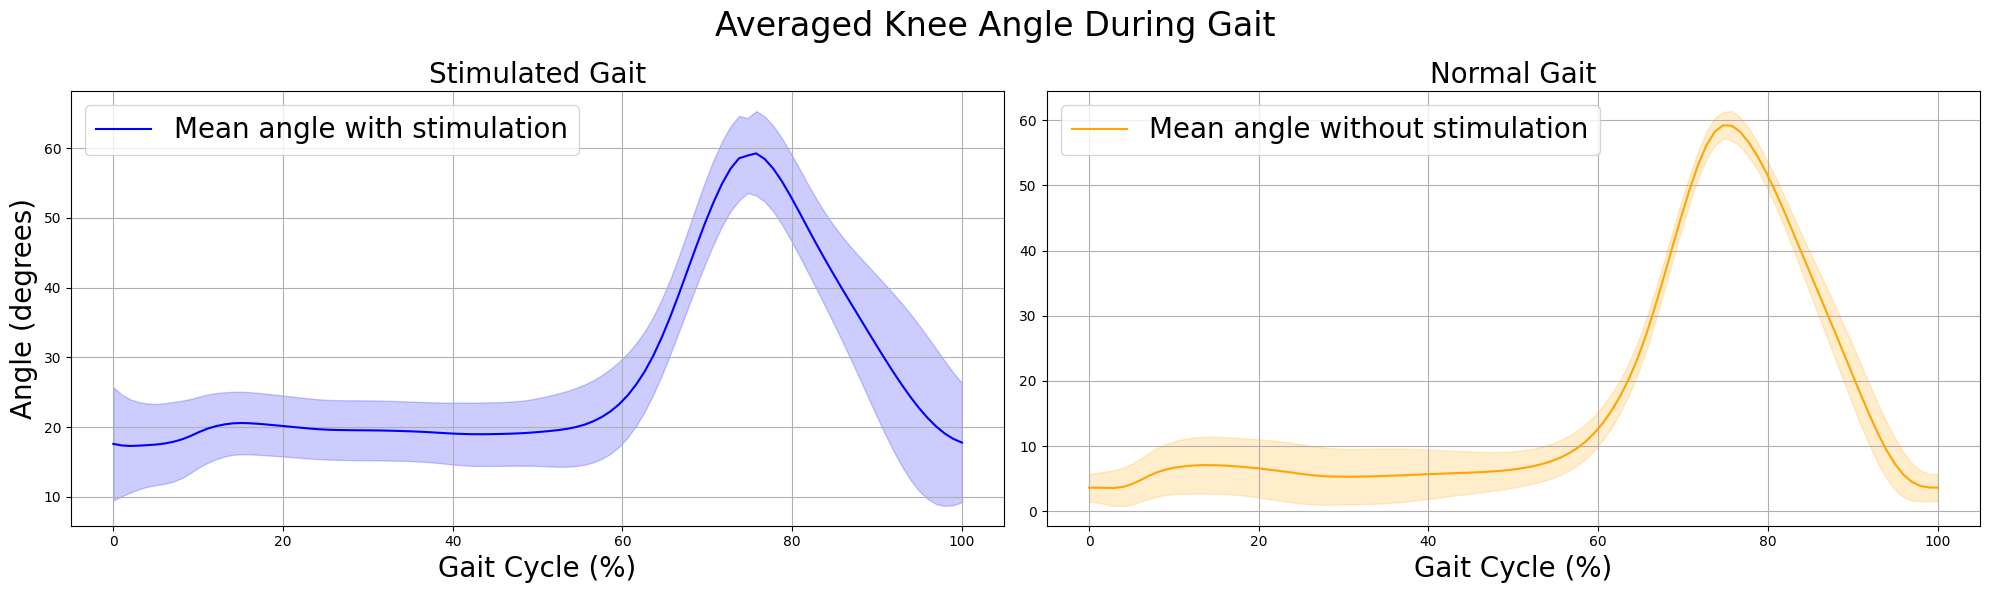
\includegraphics[width=0.99\linewidth]{images/alexisoutput1.png}
    \caption{Caption}
    \label{fig:alexisout}
\end{figure}

\begin{figure}[h]
    \centering
    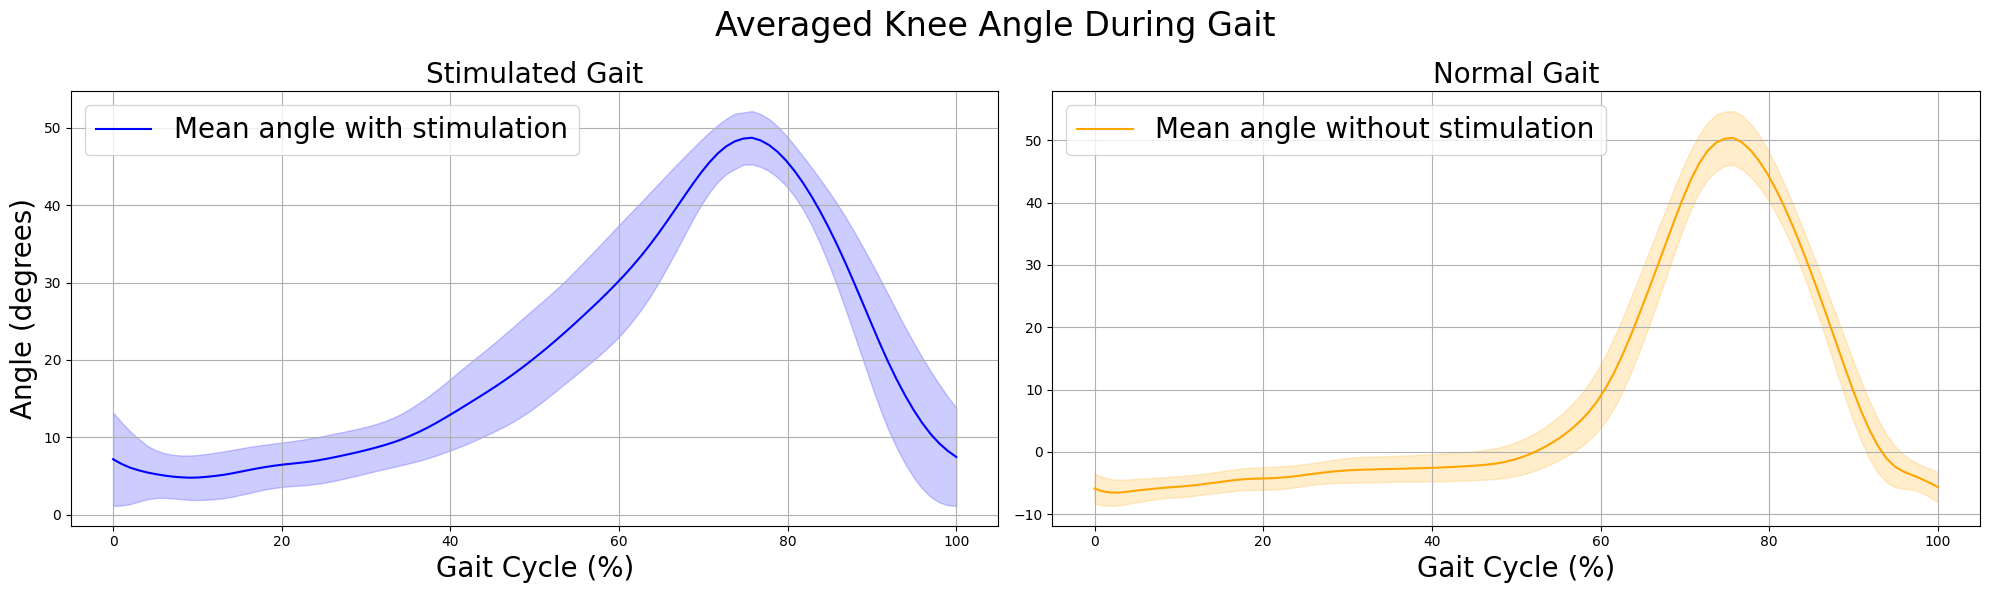
\includegraphics[width=0.99\linewidth]{images/katlaoutput1.png}
    \caption{Caption}
    \label{fig:katlaout}
\end{figure}

\begin{figure} [h]
    \centering
    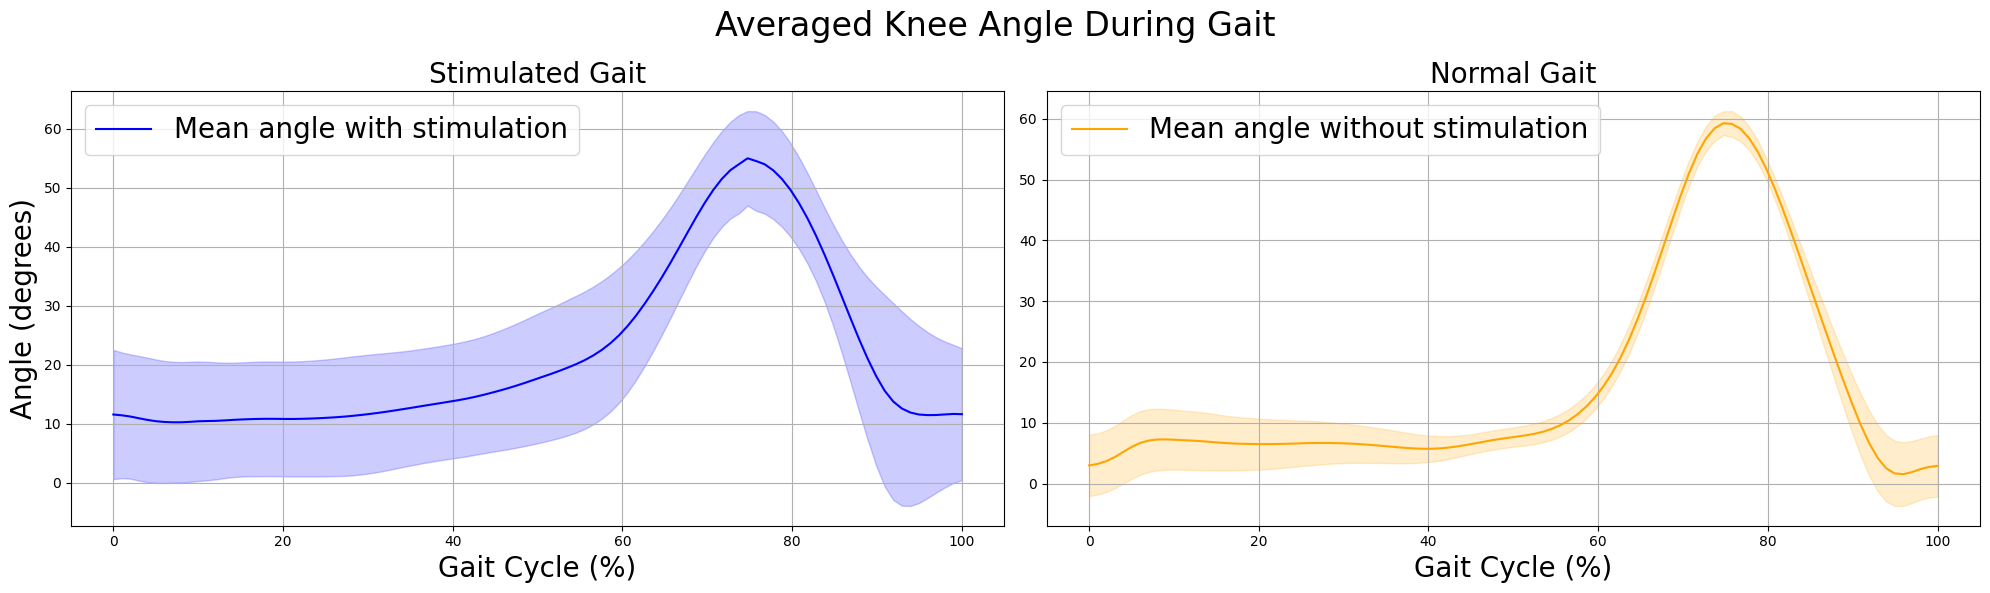
\includegraphics[width=0.99\linewidth]{images/leonioutput1.png}
    \caption{Caption}
    \label{fig:leoniout}
\end{figure}

The results from the three subjects can be seen in figure \ref{fig:alexisout}, \ref{fig:katlaout} and \ref{fig:leoniout}. A observation across all subjects is that the shapes of the mean knee angle curves are remarkably similar between the stimulated and non-stimulated conditions. This is despite natural differences in the gait patterns of the individuals. This similarity indicates that the general kinematic pattern is preserved under electrical stimulation. However, the standard deviation around is noticeably larger in the stimulated condition for all subject. Indicating increased variability in the step during stimulated walking.

One observed challenge during open-loop stimulation was that, in some instances, subjects took disproportionately small or large steps with the contralateral (non-stimulated) leg. This disrupted the gait rhythm and caused the walking pattern to fall out of sync with the stimulation pattern. Leading to instability until the subjects gait was again synchronized with the stimulation. This issue was particularly evident in subject 3 (figure \ref{fig:leoniout}), which resulted in the especially large standard deviation. This issue reflects the lack of adaptability when using an open-loop stimulation system, which does not account for real-time changes in the subject's gait rhythm or step length. 

However, overall, the results show that the open loop stimulation sequence is generalizable and works across individuals, meaning that the project could move on to further develop the closed-loop which bases its stimulation sequence on this result.

\subsection{Discussion}
\subsubsection{Analysis of the Initial Sequence}
There are several likely causes for the inaccuracies in EMG measurement that lead to the creation of the erroneous sequence, including noise, motion artifacts or inaccurate placement leading the EMG sensors to pick up activity from unintended muscles. Since the stimulation sequence was based directly on this flawed data, several muscles were being stimulated during periods where they should be entirely inactive. Additionally basing the sequence on the data of only two subjects is bound to introduce some errors due to imperfect data. This is what lead to the failure of this initial sequence in reproducing a natural and functional gait cycle. 

\subsubsection{Designing a New Sequence}
The development of the stimulation sequence was a stepwise process guided by literature, observations, and testing. This was all done with the aim of creating a simple and generalizable sequence that would work across a wide variety of subjects.

Reducing the sequence from six to four muscles addressed several challenges. Excluding the gluteus maximus improved comfort and simplified setup, as literature suggested its role in flat-ground walking could be compensated by other muscles. Removing the rectus femoris eliminated redundancy in knee extension, aligned better with its natural role during gait, and resolved issues with discomfort and electrode placement.

The final four-muscle sequence produced functional steps comparable to the six- and five-muscle sequences while being more comfortable and practical.

\subsubsection{Validation of the Final Sequence}
The results of the open loop FES highlighted the potential of sequence to produce consistent gait patterns, but there are several points that warrant discussion.
\newline

\paragraph*{Testing in Healthy individuals}

One significant challenge is the inherent difficulty of testing FES on healthy subjects. Healthy individuals naturally recruit their muscles during walking, even when instructed to minimize voluntary muscle activity and rely on stimulation. This introduces variability in the response to FES, as the subjects neuromuscular system interacts with the stimulation in ways that differ from the intended clinical scenarios. These interaction can obscure the system's true efficacy.

There are also other possible consequences. Firstly, patients with neurological impairments, there might be less of a falling out of sync issue, which observed in healthy individual in this study. The lack of competing voluntary muscle activity could make FES-induced movements more consisted and predictable. Secondly, there is evidence suggesting that patients may perceive FES differently from healthy individuals. While healthy subject often report discomfort during stimulation, patients with neurological conditions may experience reduced discomfort, potentially making it easier to achieve functional movements. This could make the setup simpler and more comfortable and effective in patient populations. \todo{source}


\paragraph*{Lack of Weight Support System}
Weight support could have created a more controlled environment for stimulation. Particularly in healthy individuals the it would have helped to minimize the effect of involuntary muscle contractions that all healthy individuals will have when placed on a treadmill. This would have lent more credibility to the results, as it is not certain how much of the movement during the gait is due only to the stimulation or if the subjects are inadvertently activating their muscles during the study.
\newline 

\paragraph*{Alignment with Natural Synergies}

The gait sequence used in this study, while not explicitly modeled on natural synergies strikingly resembles the muscle synergies during normal gait as can be seen by comparing figure and figure .

\begin{figure}[h]
    \centering
    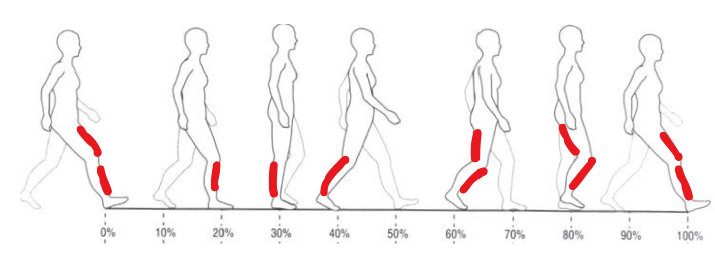
\includegraphics[width=0.9\linewidth]{images/gait_cycle_stim_seq.png}
    \caption{Final stimulation sequence}
    \label{fig:enter-label}
\end{figure}
\begin{figure} [h]
    \centering
    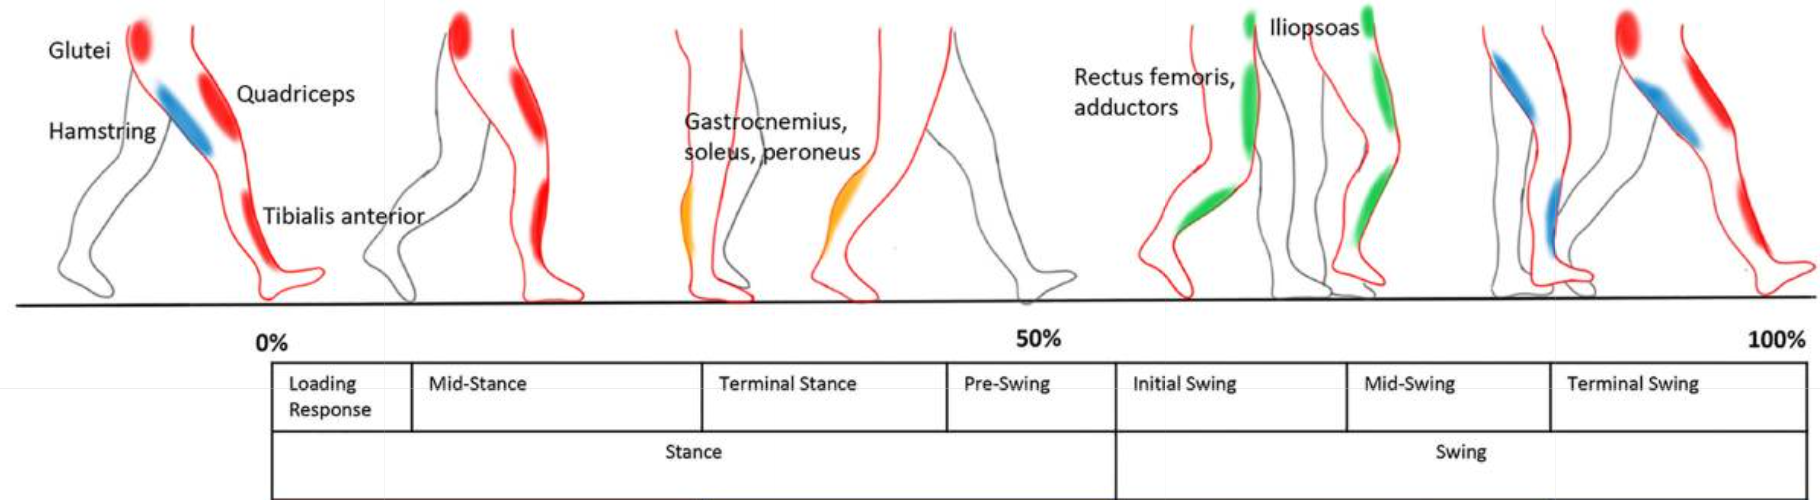
\includegraphics[width=0.9\linewidth]{images/synergies.png}
    \caption{Gait synergies \cite{magrath_systematic_2022}}
    \label{fig:enter-label}
\end{figure}


The primary deviation is in the absence of stimulation to the rectus femoris. In natural synergies, the rectus femoris plays a key role in both hip flection and knee extension \todo{source}. 

The decision to exclude rectus femoris stimulation was guided by the goal of creating a simple and comfortable sequence that is generalizable, not too complex to setup and applicable for clinical use. However, if the objective were to mimic the natural synergies, a low-current stimulation of the rectus femoris could be considered. Low current, since when stimulated it acts visibly as a knee extensor. This raises an important question about the trade offs between simplicity and fidelity to natural synergies, which should be be considered in the context of clinical goals.


\subsection{Further Work}
In future studies, incorporating a weight support system could help isolate the effects of FES on gait mechanisms and create a more controlled environment, providing a clearer assessment of its efficacy.

The findings, especially the observation of the gait falling out of sync with stimulation at times, underscores the limitations of open-loop systems and the potential advantages of closed-loop systems with real-time phase detection. By dynamically adjusting stimulation based on the current phase the consistency and functionality of the FES would be improved, resulting in a more natural and effective gait restoration



\end{document}